\subsection{littoral}
%

% - Purpose & Problem description:
%     These first two parts give reader short details about the test case,
%     the physical phenomena involved and specify how the numerical solution will be validated
%
\subsubsection{Purpose}
%
This case test the coupling model between Telemac2dTomawac and sisyphe. 
%
\subsubsection{Description of the problem}
%
THE SOLUTION IS TEPORARELLY NULL BECAUSE GEOMETRIE IS NOT GOOD (WAITING FOR JOLY'S FIX)
% - Reference:
%     This part gives the reference solution we are comparing to and
%     explicits the analytical solution when available;
%
%
\subsubsection{Reference}
%

% - Physical parameters:
%     This part specifies the geometry, details all the physical parameters
%     used to describe both porous media (soil model in particularly) and
%     solute characteristics (dispersion/diffusion coefficients, soil <=> pollutant interactions...)
%
%
\subsubsection{Physical parameters}
%

% - Geometry and Mesh:
%     This part describes the mesh used in the computation
%
%
\subsubsection{Geometry and Mesh}
%
The mesh is as shown on Figure \ref{littoralmesh}
\begin{figure} [!h]
\centering
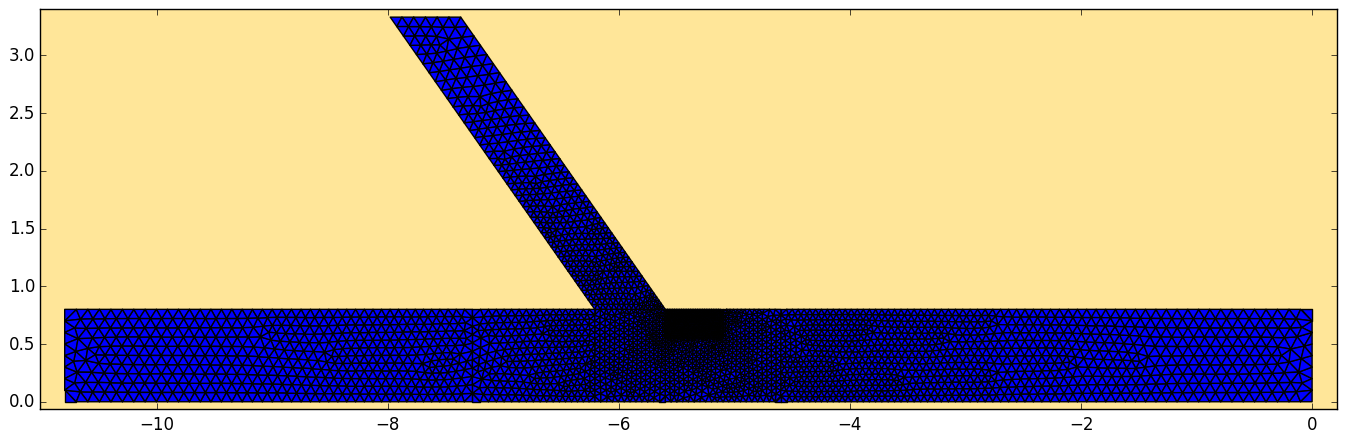
\includegraphics{../mesh.png}
 \caption{mesh of the case littoral}
\label{littoralmesh}
\end{figure}

% - Initial and boundary conditions:
%     This part details both initial and boundary conditions used to simulate the case
%
%
\subsubsection{Initial and Boundary Conditions}
%

% - Numerical parameters:
%     This part is used to specify the numerical parameters used
%     (adaptive time step, mass-lumping when necessary...)
%
%
\subsubsection{Numerical parameters}
%

% - Results:
%     We comment in this part the numerical results against the reference ones,
%     giving understanding keys and making assumptions when necessary.
%
%
\subsubsection{Results}
%
The results are presented Figures \ref{resultsT2D} (Velocity U) \ref{resultsTOM}(Wave heigth Hm0) and  \ref{resultsSIS} (Bed Shear stress)
\begin{figure} [!h]
\centering
\includegraphics{../resultsT2D.png}
 \caption{Velocity along U of the case littoral}
\label{resultsT2D}
\end{figure}
\begin{figure} [!h]
\centering
\includegraphics{../resultsTOM.png}
 \caption{Wave heigth Hm0 of the case littoral}
\label{resultsTOM}
\end{figure}
\begin{figure} [!h]
\centering
\includegraphics{../resultsSIS.png}
 \caption{Bed shear Stress of the case littoral}
\label{resultsSIS}
\end{figure}

% Here is an example of how to include the graph generated by validateTELEMAC.py
% They should be in test_case/img
%\begin{figure} [!h]
%\centering
%\includegraphics[scale=0.3]{../img/mygraph.png}
% \caption{mycaption}\label{mylabel}
%\end{figure}


